\documentclass[border=0mm]{standalone}
\usepackage[T1]{fontenc}\usepackage{helvet}\renewcommand{\familydefault}{\sfdefault}
\usepackage{tikz}
\usetikzlibrary{arrows.meta,shadings,patterns,calc,shadows.blur}
\definecolor{stahl}{HTML}{C9CED6}\definecolor{stahlh}{HTML}{E7EAEE}\definecolor{stahld}{HTML}{8A929E}
\definecolor{band}{HTML}{33373D}\definecolor{dunkel}{HTML}{1F3A5F}\definecolor{ral}{HTML}{D7DBE0}
\definecolor{motor}{HTML}{6E7F96}\definecolor{karton}{HTML}{C8975A}\definecolor{gruen}{HTML}{2E7D32}\definecolor{rot}{HTML}{C62828}
\tikzset{
 k/.style={line width=0.8pt,draw=black,line join=round},
 kf/.style={line width=0.5pt,draw=black,line join=round},
 nr/.style={circle,draw=black,fill=white,line width=0.7pt,inner sep=1pt,font=\bfseries\footnotesize,minimum size=5mm},
 hl/.style={line width=0.45pt,-{Circle[length=2pt]}},
 bmk/.style={font=\scriptsize\bfseries},
 schraube/.style={fill=stahld,draw=black,line width=0.3pt},
}
\def\dx{0.45}\def\dy{0.3}
% Quader: x y Breite Höhe Tiefe Farbe
\newcommand{\quader}[6]{%
 \fill[#6!75!black,draw=black,line width=0.8pt,line join=round] (#1+#3,#2) -- ++(#5*\dx,#5*\dy) -- ++(0,#4) -- ++(-#5*\dx,-#5*\dy) -- cycle;
 \fill[#6!45!white,draw=black,line width=0.8pt,line join=round] (#1,#2+#4) -- ++(#5*\dx,#5*\dy) -- ++(#3,0) -- ++(-#5*\dx,-#5*\dy) -- cycle;
 \shade[top color=#6!85!white,bottom color=#6,draw=black,line width=0.8pt] (#1,#2) rectangle ++(#3,#4);
 \draw[k] (#1,#2) rectangle ++(#3,#4);}

\begin{document}
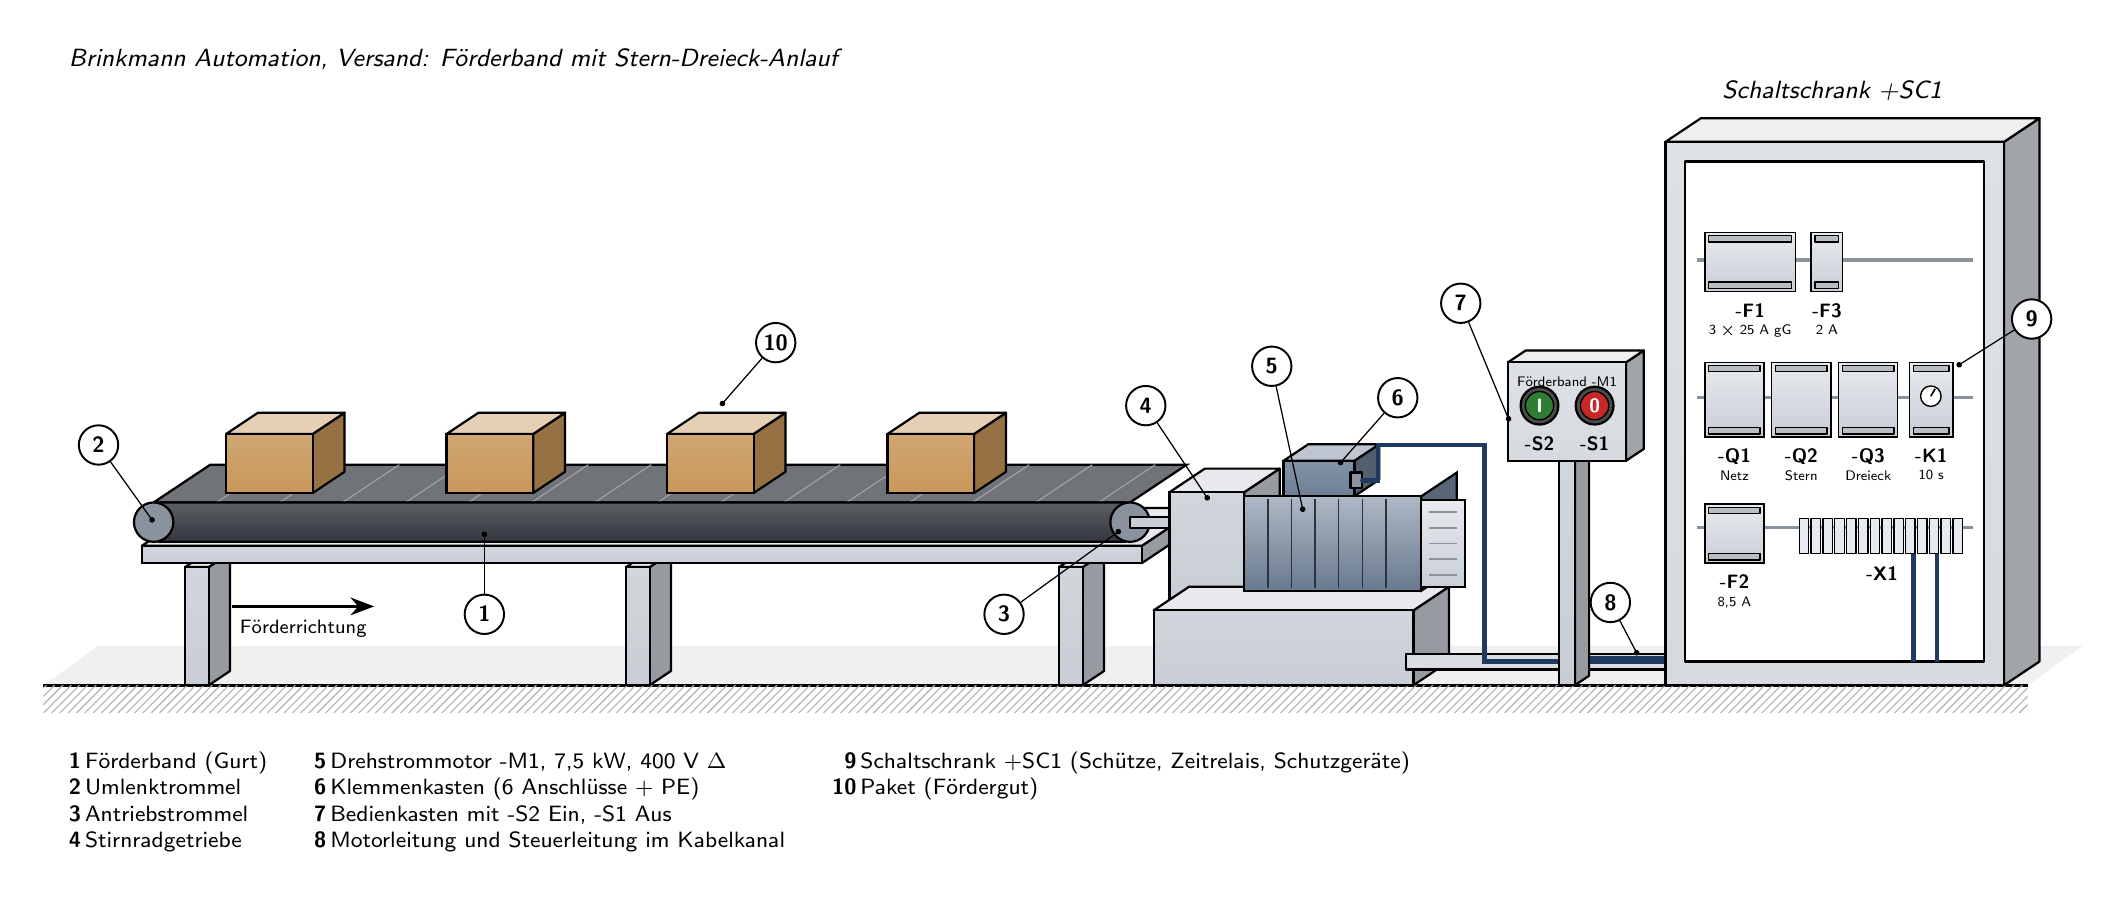
\begin{tikzpicture}[x=1cm,y=1cm]
\useasboundingbox (-1.2,-2.5) rectangle (24.8,8.3);
\fill[black!6] (-1,-0.05) -- (24.2,-0.05) -- (24.9,0.45) -- (-0.3,0.45) -- cycle;
\draw[line width=1pt] (-1,-0.05) -- (24.2,-0.05);
\fill[pattern=north east lines,pattern color=black!30] (-1,-0.4) rectangle (24.2,-0.05);
\quader{0.8}{-0.05}{0.3}{1.5}{0.6}{stahl}
\quader{6.4}{-0.05}{0.3}{1.5}{0.6}{stahl}
\quader{11.9}{-0.05}{0.3}{1.5}{0.6}{stahl}
\quader{0.25}{1.5}{12.7}{0.22}{1.6}{stahl}
\fill[band!70!white,draw=black,line width=0.8pt] (0.4,2.27) -- ++(0.72,0.48) -- (13.52,2.75) -- (12.8,2.27) -- cycle;
\draw[white!55!band,line width=0.4pt] (1.2,2.27) -- ++(0.72,0.48);
\draw[white!55!band,line width=0.4pt] (2,2.27) -- ++(0.72,0.48);
\draw[white!55!band,line width=0.4pt] (2.8,2.27) -- ++(0.72,0.48);
\draw[white!55!band,line width=0.4pt] (3.6,2.27) -- ++(0.72,0.48);
\draw[white!55!band,line width=0.4pt] (4.4,2.27) -- ++(0.72,0.48);
\draw[white!55!band,line width=0.4pt] (5.2,2.27) -- ++(0.72,0.48);
\draw[white!55!band,line width=0.4pt] (6,2.27) -- ++(0.72,0.48);
\draw[white!55!band,line width=0.4pt] (6.8,2.27) -- ++(0.72,0.48);
\draw[white!55!band,line width=0.4pt] (7.6,2.27) -- ++(0.72,0.48);
\draw[white!55!band,line width=0.4pt] (8.4,2.27) -- ++(0.72,0.48);
\draw[white!55!band,line width=0.4pt] (9.2,2.27) -- ++(0.72,0.48);
\draw[white!55!band,line width=0.4pt] (10,2.27) -- ++(0.72,0.48);
\draw[white!55!band,line width=0.4pt] (10.8,2.27) -- ++(0.72,0.48);
\draw[white!55!band,line width=0.4pt] (11.6,2.27) -- ++(0.72,0.48);
\draw[white!55!band,line width=0.4pt] (12.4,2.27) -- ++(0.72,0.48);
\shade[top color=band!80!white,bottom color=band,draw=black,line width=0.8pt,rounded corners=2pt] (0.4,1.77) rectangle (12.8,2.27);
\draw[k,fill=stahld] (0.4,2.02) circle (0.25);
\draw[k,fill=stahld] (12.8,2.02) circle (0.25);
\quader{1.32}{2.39}{1.1}{0.75}{0.9}{karton}
\quader{4.12}{2.39}{1.1}{0.75}{0.9}{karton}
\quader{6.92}{2.39}{1.1}{0.75}{0.9}{karton}
\quader{9.72}{2.39}{1.1}{0.75}{0.9}{karton}
\draw[-{Stealth[length=3mm]},line width=1pt] (1.4,0.95)--(3.2,0.95) node[midway,below=1pt,font=\scriptsize]{Förderrichtung};
\draw[k,fill=stahl] (12.8,1.95) rectangle (13.35,2.09);
\quader{13.3}{0.95}{0.95}{1.45}{1.0}{stahl}
\quader{13.1}{-0.05}{3.3}{0.95}{1.0}{stahl}
\shade[top color=motor!55,bottom color=motor!95!black,draw=black,line width=0.8pt] (14.25,1.15) rectangle (16.5,2.35);
\draw[motor!40!black,line width=0.5pt] (14.55,1.18) -- (14.55,2.32);
\draw[motor!40!black,line width=0.5pt] (14.85,1.18) -- (14.85,2.32);
\draw[motor!40!black,line width=0.5pt] (15.15,1.18) -- (15.15,2.32);
\draw[motor!40!black,line width=0.5pt] (15.45,1.18) -- (15.45,2.32);
\draw[motor!40!black,line width=0.5pt] (15.75,1.18) -- (15.75,2.32);
\draw[motor!40!black,line width=0.5pt] (16.05,1.18) -- (16.05,2.32);
\fill[motor!80!black,draw=black,line width=0.8pt] (16.5,1.15) -- ++(0.45,0.3) -- ++(0,1.2) -- ++(-0.45,-0.3) -- cycle;
\shade[top color=stahlh,bottom color=stahl,draw=black,line width=0.8pt] (16.5,1.2) rectangle (17.05,2.3);
\draw[stahld,line width=0.6pt] (16.6,1.35) -- (16.95,1.35);
\draw[stahld,line width=0.6pt] (16.6,1.55) -- (16.95,1.55);
\draw[stahld,line width=0.6pt] (16.6,1.75) -- (16.95,1.75);
\draw[stahld,line width=0.6pt] (16.6,1.95) -- (16.95,1.95);
\draw[stahld,line width=0.6pt] (16.6,2.15) -- (16.95,2.15);
\quader{14.75}{2.35}{0.9}{0.45}{0.7}{motor}
\draw[k,fill=stahld] (15.6,2.45) rectangle (15.75,2.65);
\draw[k,fill=stahl!70] (16.3,0.15) -- (19.6,0.15) -- (19.6,0.35) -- (16.3,0.35) -- cycle;
\draw[dunkel,line width=1.6pt,line cap=round] (15.75,2.55) -- (15.95,2.55) -- (15.95,3.0) -- (17.3,3.0) -- (17.3,0.25) -- (19.6,0.25);
\draw[dunkel,line width=1.2pt,line cap=round] (18.35,2.8) -- (18.35,0.3) -- (19.6,0.3);
\quader{18.25}{-0.05}{0.2}{2.85}{0.4}{stahl}
\quader{17.6}{2.8}{1.5}{1.25}{0.5}{ral}
\draw[k,fill=black!70] (18,3.5) circle (0.24);
\draw[kf,fill=gruen] (18,3.5) circle (0.18);
\node[white,font=\scriptsize\bfseries] at (18,3.5) {I};
\node[bmk,anchor=north] at (18,3.22) {-S2};
\draw[k,fill=black!70] (18.7,3.5) circle (0.24);
\draw[kf,fill=rot] (18.7,3.5) circle (0.18);
\node[white,font=\scriptsize\bfseries] at (18.7,3.5) {0};
\node[bmk,anchor=north] at (18.7,3.22) {-S1};
\node[font=\tiny] at (18.35,3.8) {Förderband -M1};
\quader{19.6}{-0.05}{4.3}{6.9}{1.0}{ral}
\draw[k,fill=white] (19.85,0.25) rectangle (23.65,6.6);
\draw[line width=1.2pt,stahld] (20.0,5.35) -- (23.5,5.35);
\draw[line width=1.2pt,stahld] (20.0,3.6) -- (23.5,3.6);
\draw[line width=1.2pt,stahld] (20.0,1.95) -- (23.5,1.95);
\shade[top color=stahlh,bottom color=stahl,draw=black,line width=0.5pt] (20.1,4.95) rectangle ++(1.15,0.75);
\draw[kf,fill=stahld!60] (20.15,5.58) rectangle ++(1.05,0.08) (20.15,4.99) rectangle ++(1.05,0.08);
\node[bmk,anchor=north] at (20.675,4.92) {-F1};
\node[font=\tiny,anchor=north] at (20.675,4.65) {3 × 25 A gG};
\shade[top color=stahlh,bottom color=stahl,draw=black,line width=0.5pt] (21.45,4.95) rectangle ++(0.4,0.75);
\draw[kf,fill=stahld!60] (21.5,5.58) rectangle ++(0.3,0.08) (21.5,4.99) rectangle ++(0.3,0.08);
\node[bmk,anchor=north] at (21.65,4.92) {-F3};
\node[font=\tiny,anchor=north] at (21.65,4.65) {2 A};
\shade[top color=stahlh,bottom color=stahl,draw=black,line width=0.5pt] (20.1,3.1) rectangle ++(0.75,0.95);
\draw[kf,fill=stahld!60] (20.15,3.93) rectangle ++(0.65,0.08) (20.15,3.14) rectangle ++(0.65,0.08);
\node[bmk,anchor=north] at (20.475,3.07) {-Q1};
\node[font=\tiny,anchor=north] at (20.475,2.8) {Netz};
\shade[top color=stahlh,bottom color=stahl,draw=black,line width=0.5pt] (20.95,3.1) rectangle ++(0.75,0.95);
\draw[kf,fill=stahld!60] (21,3.93) rectangle ++(0.65,0.08) (21,3.14) rectangle ++(0.65,0.08);
\node[bmk,anchor=north] at (21.325,3.07) {-Q2};
\node[font=\tiny,anchor=north] at (21.325,2.8) {Stern};
\shade[top color=stahlh,bottom color=stahl,draw=black,line width=0.5pt] (21.8,3.1) rectangle ++(0.75,0.95);
\draw[kf,fill=stahld!60] (21.85,3.93) rectangle ++(0.65,0.08) (21.85,3.14) rectangle ++(0.65,0.08);
\node[bmk,anchor=north] at (22.175,3.07) {-Q3};
\node[font=\tiny,anchor=north] at (22.175,2.8) {Dreieck};
\shade[top color=stahlh,bottom color=stahl,draw=black,line width=0.5pt] (22.7,3.1) rectangle ++(0.55,0.95);
\draw[kf,fill=stahld!60] (22.75,3.93) rectangle ++(0.45,0.08) (22.75,3.14) rectangle ++(0.45,0.08);
\node[bmk,anchor=north] at (22.975,3.07) {-K1};
\node[font=\tiny,anchor=north] at (22.975,2.8) {10 s};
\draw[kf,fill=white] (22.97,3.62) circle (0.13); \draw[line width=0.6pt] (22.97,3.62) -- ++(60:0.11);
\shade[top color=stahlh,bottom color=stahl,draw=black,line width=0.5pt] (20.1,1.5) rectangle ++(0.75,0.75);
\draw[kf,fill=stahld!60] (20.15,2.13) rectangle ++(0.65,0.08) (20.15,1.54) rectangle ++(0.65,0.08);
\node[bmk,anchor=north] at (20.475,1.47) {-F2};
\node[font=\tiny,anchor=north] at (20.475,1.2) {8,5 A};
\foreach \x in {21.3,21.45,...,23.3}{\draw[kf,fill=stahlh] (\x,1.62) rectangle ++(0.12,0.45);}
\node[bmk,anchor=north] at (22.35,1.57) {-X1};
\draw[dunkel,line width=1.6pt] (22.75,0.25) -- (22.75,1.62); \draw[dunkel,line width=1.2pt] (23.05,0.25) -- (23.05,1.62);
\node[font=\small\itshape,anchor=west] at (20.2,7.5) {Schaltschrank +SC1};
\node[nr] (n1) at (4.6,0.85) {1}; \draw[hl] (n1) -- (4.6,1.9);
\node[nr] (n2) at (-0.3,3) {2}; \draw[hl] (n2) -- (0.4,2.02);
\node[nr] (n3) at (11.2,0.85) {3}; \draw[hl] (n3) -- (12.68,1.92);
\node[nr] (n4) at (13,3.5) {4}; \draw[hl] (n4) -- (13.8,2.3);
\node[nr] (n5) at (14.6,4) {5}; \draw[hl] (n5) -- (15,2.15);
\node[nr] (n6) at (16.2,3.6) {6}; \draw[hl] (n6) -- (15.45,2.75);
\node[nr] (n7) at (17,4.8) {7}; \draw[hl] (n7) -- (17.62,3.3);
\node[nr] (n8) at (18.9,1) {8}; \draw[hl] (n8) -- (19.25,0.33);
\node[nr] (n9) at (24.25,4.6) {9}; \draw[hl] (n9) -- (23.3,4);
\node[nr] (n10) at (8.3,4.3) {10}; \draw[hl] (n10) -- (7.6,3.5);
\node[font=\small\itshape,anchor=west] at (-0.8,7.9) {Brinkmann Automation, Versand: Förderband mit Stern-Dreieck-Anlauf};
\node[anchor=north west,font=\footnotesize,align=left] at (-0.8,-0.75){%
\begin{tabular}{@{}r@{\,}l@{\qquad}r@{\,}l@{\qquad}r@{\,}l@{}}
\textbf{1} & Förderband (Gurt) & \textbf{5} & Drehstrommotor -M1, 7,5 kW, 400 V $\Delta$ & \textbf{9} & Schaltschrank +SC1 (Schütze, Zeitrelais, Schutzgeräte)\\
\textbf{2} & Umlenktrommel & \textbf{6} & Klemmenkasten (6 Anschlüsse + PE) & \textbf{10} & Paket (Fördergut)\\
\textbf{3} & Antriebstrommel & \textbf{7} & Bedienkasten mit -S2 Ein, -S1 Aus & &\\
\textbf{4} & Stirnradgetriebe & \textbf{8} & Motorleitung und Steuerleitung im Kabelkanal & &
\end{tabular}};
\end{tikzpicture}
\end{document}